    %\ifx\isEmbedded\undefined
%	% Loading common settings
%	\input{macros/common}
%	% Loading common variable definitions 
%	\input{macros/macros}
%	\begin{document} 
%\else
%\fi
%



\chapter{Objects}


%\section{what is an object?}
\section{A Few Notes About the History of Object Recognition Models}


representations

geometry-based models

bag of words 

part based models

appearance based models

methods

Indexing, nearest neighbors

prototypes

classifiers (matched-filters, SVMs, boosting, neural networks)



\section{A Few Notes About Object Recognition in Humans}

Object perception is very rich and diverse area of interdisciplinary research. Many of the approached in computer vision are rooted on hypothesis formulated in trying to model the mechanism used by the human visual system. It is useful to be familiar with the literature in cognitive science and neuroscience to understand the origin of existing approaches and to gain insights on how to build new models. Here we will review only a few findings, and we leave the reader with the task of going deeper into the field. 

%Through the book we have presented many ways of extracting information about the class, motion and 3D shape of an object from an image (or video). In this chapter we will focus on categorization.

\begin{comment}


\subsection{Feature integration theory}

What is an object?

- is a line an object?

- texture

- object part

- object

- group of objects

- scene


Stuff vs. objects

Things that we want to describe in images but that are neither stuff nor objects?

Object perception is highly contextual. What is

Object recognition happens under 200 ms.

\end{comment}

\begin{comment}

\subsection{Recognition by components}

%There are many theories on how humans might represent visual objects. Possibly, two of the most important ones are:

%prototypes
%components

%In 1987, Irving Biederman \cite{} introduced his recognition-by-components theory as a model of how humans recognize objects in images.   
%One important theory of object recognition by humans is the recognition-by-components theory proposed by Irving Biederman in 1987 \cite{}. 

One important theory of how humans represent and recognize objects from images is the recognition-by-components theory proposed by Irving Biederman in 1987 \cite{Biederman1987}. 
He started motivating his theory with the experiment illustrated in \fig{\ref{fig:do_it_yourself}}. Can you recognize the object depicted in the drawing? Does it look familiar?
The first observation one can make when looking at the drawing in \fig{\ref{fig:do_it_yourself}} is that it does not seem to be any object we know, instead it seems to be a made-up object that does not correspond to anything in the world. The second observation is that the object seems to be decomposable into parts and that different observers will probably make the same decomposition. The figure can be separated into parts by breaking the object in ``regions of sharp concavity''. And the third observation is that the object resembles other known objects. Does it look like an ice cream or hot-dog cart to you? 

\begin{figure}[t]
\centerline{
\includegraphics[width=0.6\linewidth]{figures/object_recognition/do_it_yourself.eps}
}
\caption{What is this? This drawing from Biederman \cite{Biederman1987}, shows a novel object. After looking at this drawing we can conclude the following: (1) we have never seen this object before, (2) it can be decomposed into parts that most people will agree with, and (3) it resembles some familiar objects. Maybe it looks like an ice cream or hot-dog cart.}
\label{fig:do_it_yourself}
\end{figure}

Biederman postulated that objects are represented by decomposing the object into a small set of geometric components (e.g., blocks, cylinders, cones, and so on.) that he called {\bf Geons}\index{Geons}. He derived 36 different Geons that were are to discriminate visually. Geons we defined by non-accidental attributes such as symmetry, colinearity, cotermination, parallelism, and curvature. An object is defined by a particular arrangement of a small set of Geons. Object recognition consists in a sequence of stages: (1) edge detection, (2) detection of non-accidental properties, (3) detection of Geons, and (4) matching the detected Geons to stored object representations.

One important aspect of this theory is that objects are formed by  compositing simpler elements (Geons), which are shared across many different object classes. 
{\bf Compositionality} in the visual world is not as strong as the one found in language, where a fix set of words are composed to form sentences with different meanings. In the visual world, components shared across different object classes will have different visual appearances (e.g., legs of tables and chairs share many properties but are not identical).
Geons are great to represent artificial objects (e.g., tables, cabinets, and phones) but fail when applied to represent stuff (e.g., grass, clouds, and water) or highly textured objects such as trees or food. 

Decomposing an object into parts has been an important ingredient of many computer vision object recognition systems \cite{Felzenszwalb2010,Fischler1973,Weber2000}. 

\subsection{Invariances}

Object recognition in humans seems to be quite robust to changes in viewpoint, illumination, occlusion, deformations, styles, and so on. However, perception is not completely invariant to those variables.

One well studied property of the human visual system is its invariance to image and 3D rotations.  As we discussed in \chap{\ref{chapter:bias_and_shift}}, studies in human visual perception have shown that objects are recognized faster when they appear in canonical poses. 

%Mental rotation has been thoroughly studied in cognitive science. 
In a landmark study, Roger N. Shepard and Jaqueline Metzler \cite{Shepard1971aa} showed to participants pairs of drawings of three-dimensional objects (\fig{\ref{fig:mental_rotation}}). The pair of drawings could show the same object with a mirror or the same object with an arbitrary 3D rotation. The task consisted in deciding if the two objects were identical (up to a 3D rotation) or mirror images of each other. During the experiment, they recorded the success rate and the reaction time (how long did participant took to answer). The result showed that participants had a reaction time proportional to the rotation angle between the two views. This supported the idea that participants were performing a {\bf mental rotation} in order to compare both views. Whether humans actually perform mental rotations or not still remains controversial. 


\begin{figure}
\centerline{

\includegraphics[width=0.6\linewidth]{figures/object_recognition/mental_rotation.eps}
}
\caption{Two figures related by a 3D rotation. Modified from \cite{Shepard1971aa}.}
\label{fig:mental_rotation}
\end{figure}

Michael Tarr and Steven Pinker \cite{Tarr1989MentalRA} showed that similar results where obtained on a learning task. When observers learn to recognize a novel object from a single viewpoint they are able to generalize to new viewpoints but they do that at a cost: recognition time increases with the angle of rotation as if they had to mentally rotate the object in order to compare it with the view viewed during training. When trained with multiple viewpoints, participants recognized equally quickly all the familiar orientations. 

The field of cognitive science has formulated a number hypothesis about the mechanisms used for recognizing objects: geometry based models, view-based templates, prototypes, and so on. Many of those hypothesis have been the inspiration for computer vision approaches for object recognition. 



%When subjects were trained with images of the object on a single viewpoint, 

%``With practice, subjects recognized the objects almost equally quickly at all the familiar orientations.''

%Tarr MJ, Pinker S. 1989. Mental rotation and orientation-dependence in shape recognition. Cogn. Psychol. 21:233–82


%When we are presented with a novel object, we can learn its properties from a single viewpoint, but recognizing the object when it appears with a different orientation takes longer. In fact, the time it takes to compare two different versions of the object grows linearly with the angle between both viewpoints. 

\subsection{Principles of Categorization}

When working on object recognition, one typical task is to train a classifier to classify images of objects into categories. A category represents a collection of equivalent objects. Categorization offers a number of advantages. As described in \cite{Rosch1976BasicOI} ``It is to the organism’s advantage not to differentiate one stimulus from others when that differentiation is irrelevant for the purposes at hand.'' Eleanor Rosch and her collaborators proposed that categorization occurred at there different levels of abstraction: superordinate level, basic-level, and subordinate level. The following example, from \cite{Rosch1978}, illustrates the three different levels of categorization:
\begin{table}[h]
\marginnote{{\bf Table \ref{table:levels_of_categorization}}: Confusion matrix for a three-way classification task. The numbers are percentages. } 
\faketablecaption{} 
\label{table:levels_of_categorization}
\begin{center}
\begin{tabular}{l|l|l}
Superordinate & Basic Level & Subordinate\\
\cline{1-3}
Furniture & Chair & Kitchen chair\\
 &  & Living-room chair\\
 & Table & Kitchen table\\
 & & Dining-room table\\
 & Lamp & Floor lamp\\
 & & Desk lamp\\
Tree & Oak & White oak\\
 & & Red oak\\
 & Maple & Silver maple\\
 & & Sugar maple\\
 & Birch & River birch\\
 & & White birch\\
\end{tabular}
\end{center}
\end{table}

Object categorization into discrete classes has been a dominant approach in computer vision. One example is the ImageNet dataset that organizes categories into the taxonomy introduced by WordNet \cite{Fellbaum1998}. 


However, as argued by E. Rosch \cite{Rosch1978}, ``natural categories tend to be fuzzy at their boundaries and inconsistent in the status of their constituent members.'' Rosch suggested that categories can be represented by {\bf prototypes}. Prototypes are the clearest members of a category. Rosch hypothesized that humans recognize categories by measuring the similarity to prototypes. 
By using prototypes, Rosch \cite{Rosch1978} suggested that it is easier to work with continuous categories, as the categories are defined by the ``clear cases rather than its boundaries.''








%    Superordinate level: Superordinate categories are the most general ones. They are the ones that are at the top of a folk taxonomy).
%    Basic, or generic, level: categories at the basic, or middle, level are perceptually and conceptually the more salient. The generic level of a category tends to elicit the most responses and richest images, providing a basic gestalt, and seems to be the psychologically basic level. Basic level categories are members of superordinate level categories.
%    Subordinate level: Subordinate level categories are the most specific ones. They are the members of the basic level categories. They have clearly identifiable gestalts and many individuating specific features.

    







But object recognition is not as straightforward as a categorization task and using categories can result in a number of issues. One example is dealing with the different affordances that an object might have as a function of context.
In language, a word or a sentence can have a standing meaning and an occasion meanings. An standing meaning corresponds to the conventional meaning of an expression. The occasion meaning is the particular meaning that the same expression might have when used in a specific context. Therefore, when an expression is being used, it has an occasion meaning that differs from its conventional meaning. The same thing happens with visual objects as illustrated in \fig{\ref{fig:box_table}}.

\begin{figure}
\centerline{
\sublabel{a}{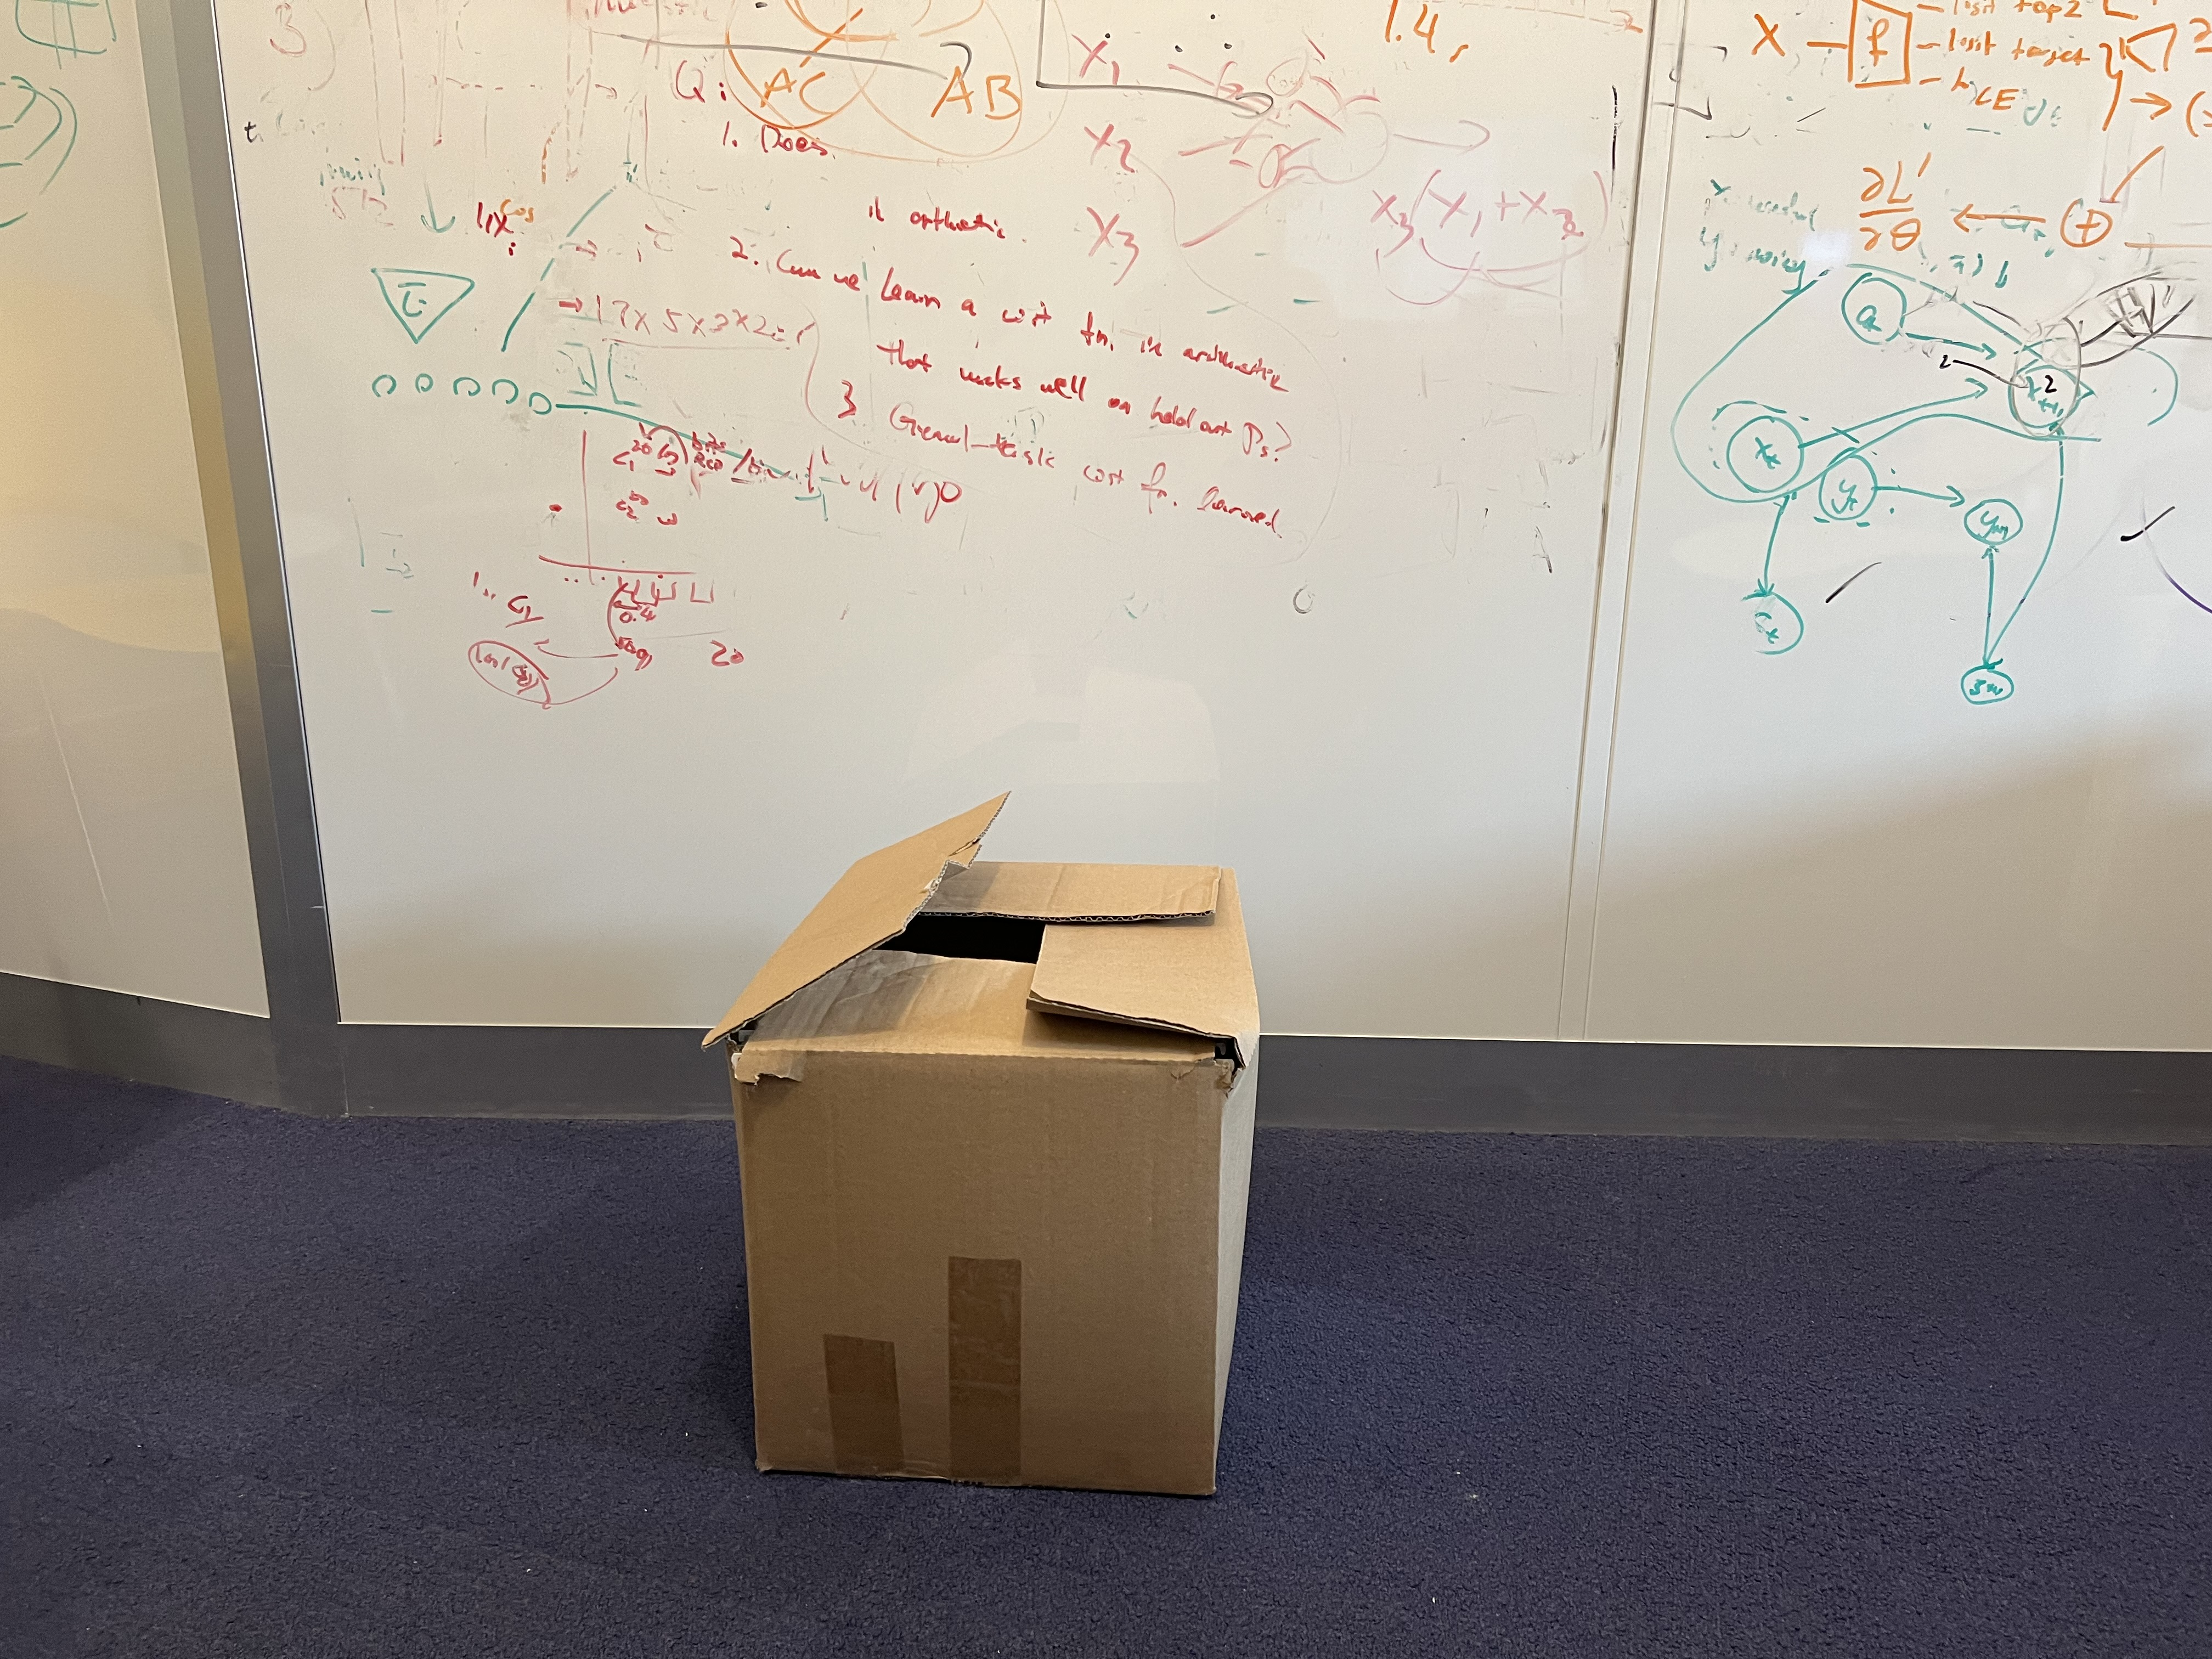
\includegraphics[width=0.475\linewidth]{figures/object_recognition/box_box2.jpg}}
\sublabel{b}{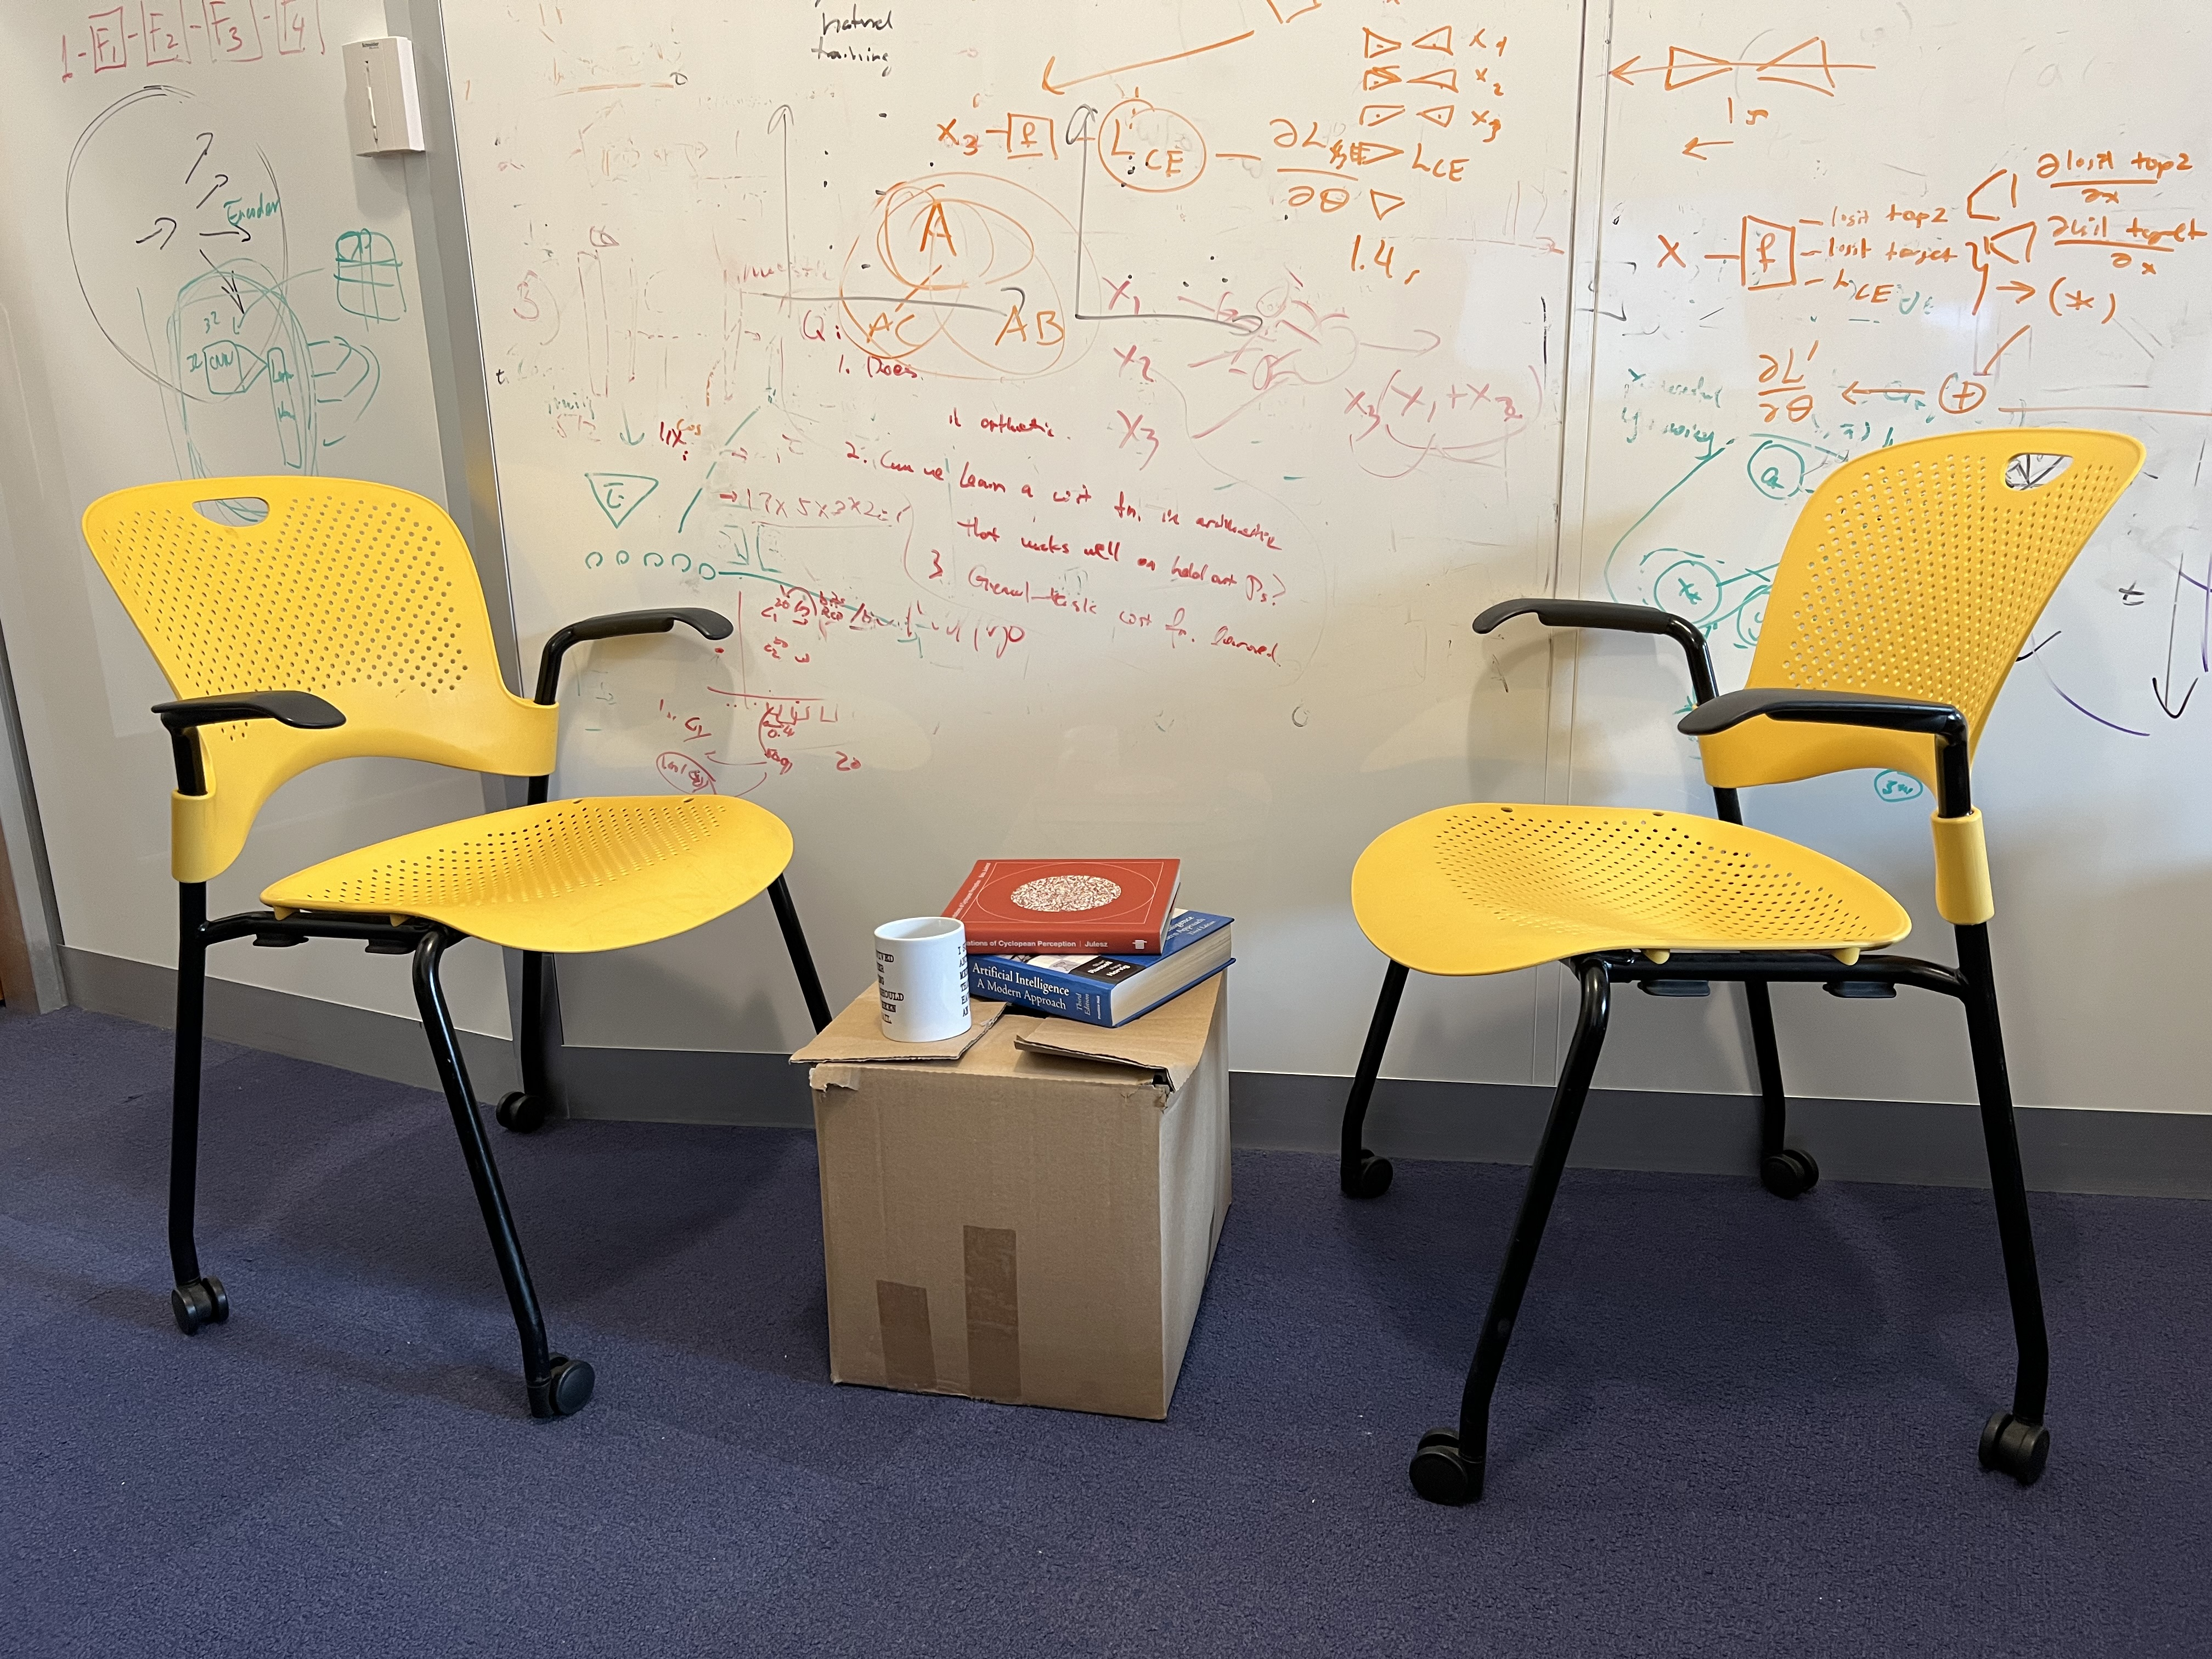
\includegraphics[width=0.475\linewidth]{figures/object_recognition/box_table.jpg}}
}
\caption{The same object can have different occasion meanings depending on the context. (a) A box. (b) A box used as a table.}
\label{fig:box_table}
\end{figure}

Avoinding categorization all together has been also the focus on some computer vision approaches to image understanding like {\bf the Visual Memex} by Malisiewicz and Efros \cite{malisiewicz-nips09}.




%The specific meaning of a word is defined by the surrounding context in which the word  is used.

%So we can say that objects have a common affordance, but the affordance might change  depending  on context. If we use  a box as a table, we might still call it "a box" but we understand the scene in a different way.   

%FIGURE: two chairs around a coffee table, two chairs around a box, two chairs around an open box and  the chairs have glasses being unpacked on top of them. 
\end{comment}

\begin{comment}

\subsection{Neural basis of object recognition}

Reading neural data with fmri and translating it into pictures. 

parahippocampal place area (PPA)

``Kanwisher N, McDermott J, Chun MM. 1997. The fusiform face area: a module in
human extrastriate cortex specialized for face perception. J. Neurosci. 17(11):4302–11''

``(Gross and Bender
1969, Gross et al. 1972) reported that neurons
in the inferotemporal (IT) cortex of macaques
responded most strongly to complex visual
stimuli, such as hands and faces.''

``suggest a
sparse, distributed code that, when uncovered
by neurophysiology, is capable of providing
constraint on how objects come to be both
represented and recognized.''

Tanaka
(1996).

``Tanaka used an
image-reduction technique on a neuron-byneuron
basis to determine which combination
of minimal image features maintains the same
firing rate as that measured in response to a
complex object image for which a given neuron
is preferential. These single-neuron object
preferences were established by rapidly
presenting a large number of common objects
to anesthetized monkeys.''





\section{Concluding remarks}

Object recognition in computer vision focuses on language (captioning, tagging, ...). This makes difficult to deal with new objects that we have never seen before. 

What can we do besides associating an object with a word.
\begin{itemize}
\item Is it familiar? What are other similar objects I know?
\item What is its 3D shape?
\item is this piece of matter an object? could I find other instances that might belong to the same class or is it just a random arrangement of things with little chances of being found somewhere else?
\item What are its mechanical properties. Is it soft, does it has parts, is it rigid, or deformable?
\item Is it resting on the ground? How is it supported? 
\item What might this object be useful for? if I have to solve a task, can I use this object?
\item How will it react to external actions?
\item Can I grasp the object? how? 
\item Is it alive? Can I eat it?
\item What is the physical process that created it? Is it man-made or  natural? How did the object arrived to its current location? 
\end{itemize}

Those are the questions that scientist would ask about when observing a new natural phenomena. The visual system will behave as a scientist when confronted with a new visual stimuli. It will formulate hypothesis and it will analyze the visual input, devise experiments and perform interventions to answer them. One can use language to answer those questions, but language does not need to be the internal representation used.






Theories of object perception
		What is an object?
			Object perception is one of  the most important functions of the visual system. 
			The visual system process objects in 150ms,  which  is amazing because  if one counts the number of neural layers  from the receptors to the decision center, there  is barely time to have one spike per neuron. 
			
		Categories
			Most work in computer vision focuses on categories. 
			Definition of a category. FIGURE: show a category tree. 
			Show different tables, until it is not clear any more if it is a table:  Interesting  analogy in language "expressions have a standing meaning fixed by convention and known to those who are linguistically competent. On the other hand, expressions in use are associated with occasion meanings which is discerned by interpreters in part on the basis of contextual information. The terminology is from Quine (1960). Kaplan (1977) uses the terms character and content". So we can say that objects have a common affordance, but the affordance might change  depending  on context. If we use  a box as a table, we might still call it "a box" but we understand the scene in a different way.   
			FIGURE: two chairs around a coffee table, two chairs around a box, two chairs around an open box and  the chairs have glasses being unpacked on top of them. 
			
		Levels of categorization
		
		
		% useful link: https://plato.stanford.edu/entries/compositionality/

\section{Why is object recognition difficult?} 

Intrinsic changes:
\begin{itemize}
    \item Changes in viewpoint
    \item Changes in scale
    \item Changes in style and appearance
\end{itemize}

Extrinsic changes:
\begin{itemize}
    \item Changes in illumination
    \item Complex background, which similar statistics than the objects themselves. Objects are made of edges, textures, just like the background is. Objects are rarely in front of a flat background. 
    \item Occlusions
\end{itemize}

Objects live in a 3D world, but we only observe 2D images of them.

	Why is detecting objects difficult: 
		FIGURE: I like josh example of learning from one example to detect a very strange object
		Rigid objects, objects made of rigid parts, deformable objects
		challenges: deformation, illumination, degradations, styles, occlusions

- notions from psy
- categorization and why it is useful. Wordnet tree.
- boundaries are not so clear

- Compositionality: scenes -> objects -> parts

- invariances

why we need a learning based system? because diversity is too wild. 

\section{What is an object?} 





\end{comment}
